\subsection{RGB-D Camera Model}

Compared to binocular cameras that calculate depth by parallax, RGB-D cameras are more "active" and can actively measure the depth of each pixel. The current RGB-D cameras can be divided into two categories according to the principle (see \autoref{fig:RGBDCamera}~):

\begin{enumerate}
	\item measures pixel distance by \textbf{Structured Light}. Examples are Kinect 1 generation, Project Tango 1 generation, Intel RealSense and so on.
	\item measures the pixel distance by the \textbf{Time-of-flight (ToF)} principle. Examples are the Kinect 2 generation and some existing ToF sensors.
\end{enumerate}

\begin{figure}[!ht]
	\centering
	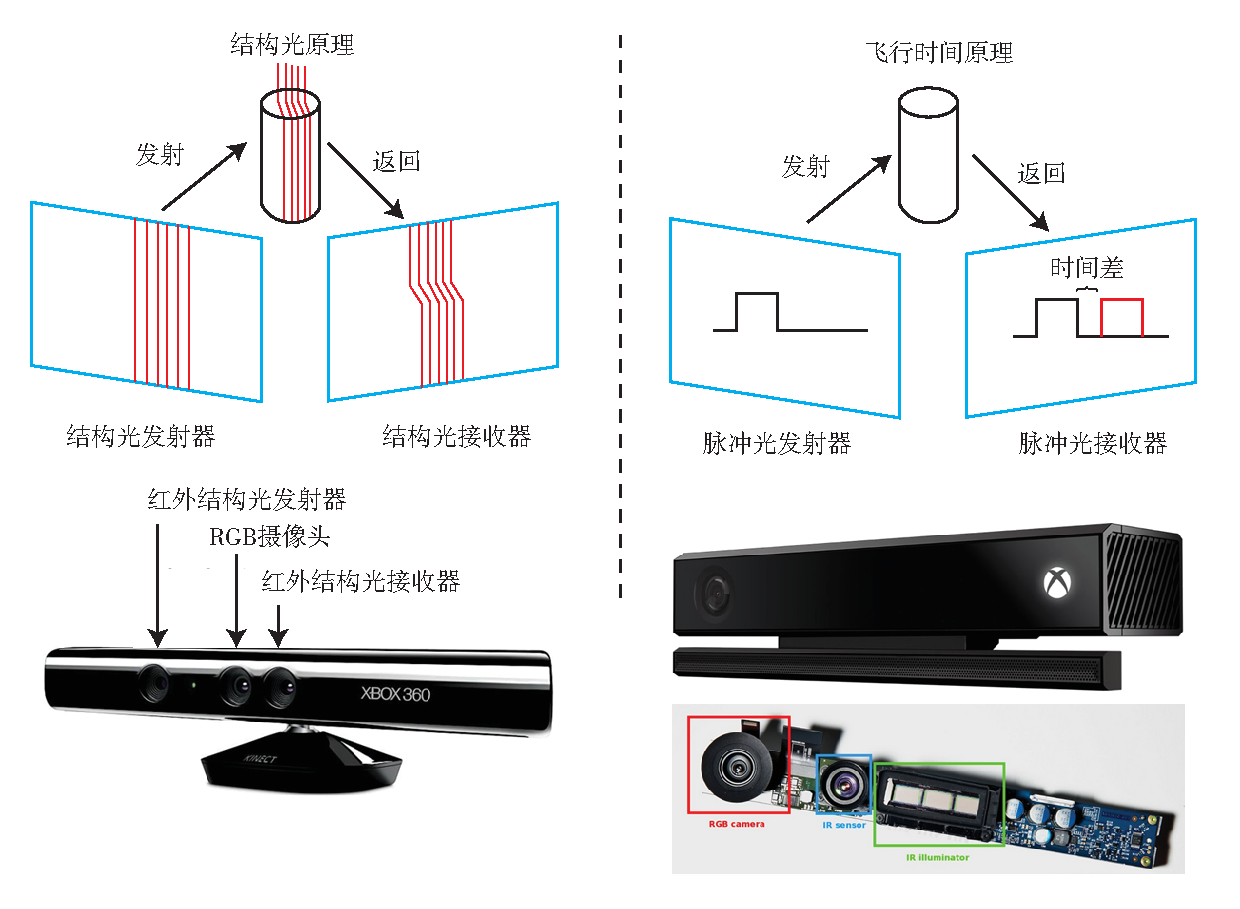
\includegraphics[width=1.0 \ textwidth]{chapter05/resources/cameraModel/rgbdCamera.pdf}
	\caption{Figure RGB-D camera schematic. }
	\label{fig:RGBDCamera}
\end{figure}

Regardless of the type, the RGB-D camera needs to emit a beam of light (usually infrared light) to the detection target. In the structured light principle, the camera calculates the distance between the object and itself based on the returned structured light pattern. In the ToF principle, the camera emits pulsed light to the target and then determines the distance between the object and itself based on the time of flight of the beam between the transmissions and the return. The ToF principle is very similar to the laser sensor, except that the laser acquires the distance by point-by-point scanning, while the ToF camera can obtain the pixel depth of the entire image, which is the characteristic of the RGB-D camera. So, if you take apart an RGB-D camera, you will usually find at least one transmitter and one receiver in addition to the normal camera.

After measuring the depth, the RGB-D camera usually completes the pairing between the depth and the color map pixels according to the position of each camera at the time of production, and outputs a one-to-one corresponding color map and depth map. We can read the color information and distance information in the same image position, calculate the 3D camera coordinates of the pixel, and generate a Point Cloud. For RGB-D data, it can be processed at the image level or at the point cloud level. The second experiment in this talk will demonstrate the point cloud construction process for RGB-D cameras.

The RGB-D camera measures the distance of each pixel in real time. However, due to this type of emission-receiving measurement, its range of use is limited. RGB-D cameras that use infrared light for depth measurement are susceptible to interference from sunlight or other sensors and therefore cannot be used outdoors. In the absence of modulation, simultaneous use of multiple RGB-D cameras can also interfere with each other. For objects with a transmissive material, the position of these points cannot be measured because no reflected light is received. In addition, RGB-D cameras have some disadvantages in terms of cost and power consumption.

% TODO Fisheye Camera Model